% Options for packages loaded elsewhere
\PassOptionsToPackage{unicode}{hyperref}
\PassOptionsToPackage{hyphens}{url}
%
\documentclass[
]{book}
\usepackage{amsmath,amssymb}
\usepackage{lmodern}
\usepackage{iftex}
\ifPDFTeX
  \usepackage[T1]{fontenc}
  \usepackage[utf8]{inputenc}
  \usepackage{textcomp} % provide euro and other symbols
\else % if luatex or xetex
  \usepackage{unicode-math}
  \defaultfontfeatures{Scale=MatchLowercase}
  \defaultfontfeatures[\rmfamily]{Ligatures=TeX,Scale=1}
\fi
% Use upquote if available, for straight quotes in verbatim environments
\IfFileExists{upquote.sty}{\usepackage{upquote}}{}
\IfFileExists{microtype.sty}{% use microtype if available
  \usepackage[]{microtype}
  \UseMicrotypeSet[protrusion]{basicmath} % disable protrusion for tt fonts
}{}
\makeatletter
\@ifundefined{KOMAClassName}{% if non-KOMA class
  \IfFileExists{parskip.sty}{%
    \usepackage{parskip}
  }{% else
    \setlength{\parindent}{0pt}
    \setlength{\parskip}{6pt plus 2pt minus 1pt}}
}{% if KOMA class
  \KOMAoptions{parskip=half}}
\makeatother
\usepackage{xcolor}
\IfFileExists{xurl.sty}{\usepackage{xurl}}{} % add URL line breaks if available
\IfFileExists{bookmark.sty}{\usepackage{bookmark}}{\usepackage{hyperref}}
\hypersetup{
  pdftitle={SIDS-Related Mortality in Cook County, IL},
  pdfauthor={Daniel P. Hall Riggins},
  hidelinks,
  pdfcreator={LaTeX via pandoc}}
\urlstyle{same} % disable monospaced font for URLs
\usepackage{color}
\usepackage{fancyvrb}
\newcommand{\VerbBar}{|}
\newcommand{\VERB}{\Verb[commandchars=\\\{\}]}
\DefineVerbatimEnvironment{Highlighting}{Verbatim}{commandchars=\\\{\}}
% Add ',fontsize=\small' for more characters per line
\usepackage{framed}
\definecolor{shadecolor}{RGB}{248,248,248}
\newenvironment{Shaded}{\begin{snugshade}}{\end{snugshade}}
\newcommand{\AlertTok}[1]{\textcolor[rgb]{0.94,0.16,0.16}{#1}}
\newcommand{\AnnotationTok}[1]{\textcolor[rgb]{0.56,0.35,0.01}{\textbf{\textit{#1}}}}
\newcommand{\AttributeTok}[1]{\textcolor[rgb]{0.77,0.63,0.00}{#1}}
\newcommand{\BaseNTok}[1]{\textcolor[rgb]{0.00,0.00,0.81}{#1}}
\newcommand{\BuiltInTok}[1]{#1}
\newcommand{\CharTok}[1]{\textcolor[rgb]{0.31,0.60,0.02}{#1}}
\newcommand{\CommentTok}[1]{\textcolor[rgb]{0.56,0.35,0.01}{\textit{#1}}}
\newcommand{\CommentVarTok}[1]{\textcolor[rgb]{0.56,0.35,0.01}{\textbf{\textit{#1}}}}
\newcommand{\ConstantTok}[1]{\textcolor[rgb]{0.00,0.00,0.00}{#1}}
\newcommand{\ControlFlowTok}[1]{\textcolor[rgb]{0.13,0.29,0.53}{\textbf{#1}}}
\newcommand{\DataTypeTok}[1]{\textcolor[rgb]{0.13,0.29,0.53}{#1}}
\newcommand{\DecValTok}[1]{\textcolor[rgb]{0.00,0.00,0.81}{#1}}
\newcommand{\DocumentationTok}[1]{\textcolor[rgb]{0.56,0.35,0.01}{\textbf{\textit{#1}}}}
\newcommand{\ErrorTok}[1]{\textcolor[rgb]{0.64,0.00,0.00}{\textbf{#1}}}
\newcommand{\ExtensionTok}[1]{#1}
\newcommand{\FloatTok}[1]{\textcolor[rgb]{0.00,0.00,0.81}{#1}}
\newcommand{\FunctionTok}[1]{\textcolor[rgb]{0.00,0.00,0.00}{#1}}
\newcommand{\ImportTok}[1]{#1}
\newcommand{\InformationTok}[1]{\textcolor[rgb]{0.56,0.35,0.01}{\textbf{\textit{#1}}}}
\newcommand{\KeywordTok}[1]{\textcolor[rgb]{0.13,0.29,0.53}{\textbf{#1}}}
\newcommand{\NormalTok}[1]{#1}
\newcommand{\OperatorTok}[1]{\textcolor[rgb]{0.81,0.36,0.00}{\textbf{#1}}}
\newcommand{\OtherTok}[1]{\textcolor[rgb]{0.56,0.35,0.01}{#1}}
\newcommand{\PreprocessorTok}[1]{\textcolor[rgb]{0.56,0.35,0.01}{\textit{#1}}}
\newcommand{\RegionMarkerTok}[1]{#1}
\newcommand{\SpecialCharTok}[1]{\textcolor[rgb]{0.00,0.00,0.00}{#1}}
\newcommand{\SpecialStringTok}[1]{\textcolor[rgb]{0.31,0.60,0.02}{#1}}
\newcommand{\StringTok}[1]{\textcolor[rgb]{0.31,0.60,0.02}{#1}}
\newcommand{\VariableTok}[1]{\textcolor[rgb]{0.00,0.00,0.00}{#1}}
\newcommand{\VerbatimStringTok}[1]{\textcolor[rgb]{0.31,0.60,0.02}{#1}}
\newcommand{\WarningTok}[1]{\textcolor[rgb]{0.56,0.35,0.01}{\textbf{\textit{#1}}}}
\usepackage{longtable,booktabs,array}
\usepackage{calc} % for calculating minipage widths
% Correct order of tables after \paragraph or \subparagraph
\usepackage{etoolbox}
\makeatletter
\patchcmd\longtable{\par}{\if@noskipsec\mbox{}\fi\par}{}{}
\makeatother
% Allow footnotes in longtable head/foot
\IfFileExists{footnotehyper.sty}{\usepackage{footnotehyper}}{\usepackage{footnote}}
\makesavenoteenv{longtable}
\usepackage{graphicx}
\makeatletter
\def\maxwidth{\ifdim\Gin@nat@width>\linewidth\linewidth\else\Gin@nat@width\fi}
\def\maxheight{\ifdim\Gin@nat@height>\textheight\textheight\else\Gin@nat@height\fi}
\makeatother
% Scale images if necessary, so that they will not overflow the page
% margins by default, and it is still possible to overwrite the defaults
% using explicit options in \includegraphics[width, height, ...]{}
\setkeys{Gin}{width=\maxwidth,height=\maxheight,keepaspectratio}
% Set default figure placement to htbp
\makeatletter
\def\fps@figure{htbp}
\makeatother
\setlength{\emergencystretch}{3em} % prevent overfull lines
\providecommand{\tightlist}{%
  \setlength{\itemsep}{0pt}\setlength{\parskip}{0pt}}
\setcounter{secnumdepth}{5}
\usepackage{booktabs}
\ifLuaTeX
  \usepackage{selnolig}  % disable illegal ligatures
\fi
\usepackage[]{natbib}
\bibliographystyle{apalike}

\title{SIDS-Related Mortality in Cook County, IL}
\author{Daniel P. Hall Riggins}
\date{2022-02-20}

\begin{document}
\maketitle

{
\setcounter{tocdepth}{1}
\tableofcontents
}
\hypertarget{sids-related-mortality-in-cook-county-il}{%
\chapter{SIDS-Related Mortality in Cook County, IL}\label{sids-related-mortality-in-cook-county-il}}

\hypertarget{about}{%
\section{About}\label{about}}

This analysis seeks to describe, map, and model the number of Sudden Infant Death Syndrome (SIDS)-related deaths in Cook County, IL census tracts for the purposes of public health interventions.

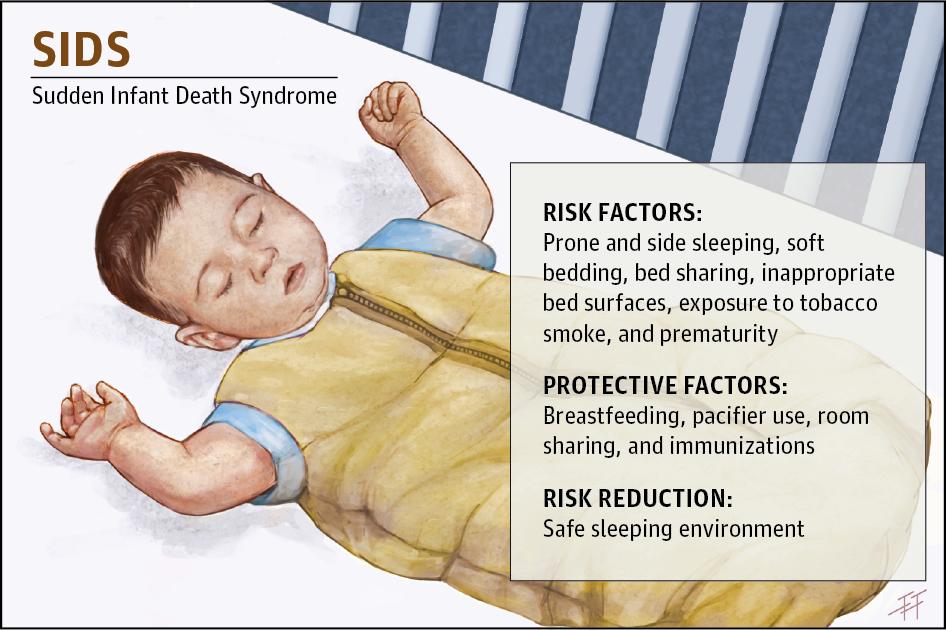
\includegraphics[width=13.14in]{media/safe_sleep}

\emph{Image credit to \href{https://jamanetwork.com/journals/jamapediatrics/fullarticle/2599897}{JAMA Pediatrics}}

\hypertarget{import-the-data}{%
\chapter{Import the Data}\label{import-the-data}}

\hypertarget{dependencies}{%
\section{Dependencies}\label{dependencies}}

\begin{Shaded}
\begin{Highlighting}[]
\CommentTok{\# Load needed modules}
\NormalTok{box}\SpecialCharTok{::}\FunctionTok{use}\NormalTok{(}
\NormalTok{    dplyr[full\_join, glimpse, select],}
\NormalTok{    janitor[clean\_names],}
\NormalTok{    magrittr[}\StringTok{\textasciigrave{}}\AttributeTok{\%\textgreater{}\%}\StringTok{\textasciigrave{}}\NormalTok{],}
\NormalTok{    readxl[read\_xlsx],}
\NormalTok{    sf[st\_set\_geometry],}
    \AttributeTok{sids\_data\_wrangling =}\NormalTok{ .}\SpecialCharTok{/}\NormalTok{modules}\SpecialCharTok{/}\NormalTok{sids\_data\_wrangling,}
\NormalTok{    tibble[as\_tibble]}
\NormalTok{)}
\end{Highlighting}
\end{Shaded}

\hypertarget{initial-import}{%
\section{Initial import}\label{initial-import}}

First, read in the excel file that was originally shared for this project:

\begin{Shaded}
\begin{Highlighting}[]
\NormalTok{raw }\OtherTok{\textless{}{-}} 
    \CommentTok{\# Parse excel file}
    \FunctionTok{read\_xlsx}\NormalTok{(}\StringTok{"data/finaldataforanalysis3\_220121.xlsx"}\NormalTok{) }\SpecialCharTok{\%\textgreater{}\%}
    \CommentTok{\# Clean up variability in naming conventions}
    \FunctionTok{clean\_names}\NormalTok{()}
\end{Highlighting}
\end{Shaded}

\hypertarget{join-census-tract-populations}{%
\section{Join census tract populations}\label{join-census-tract-populations}}

Then, import census population data:

\begin{Shaded}
\begin{Highlighting}[]
\DocumentationTok{\#\# This is a custom function I wrote that }
\DocumentationTok{\#\# pulls data from the TidyCensus API about}
\DocumentationTok{\#\# the population count of people under five }
\DocumentationTok{\#\# years old and about spatial features }
\DocumentationTok{\#\# for each census tract. I have commented it }
\DocumentationTok{\#\# out and saved the result in an RDS file}
\DocumentationTok{\#\# so as to not make a new call to the API }
\DocumentationTok{\#\# every time this script is run. You can}
\DocumentationTok{\#\# inspect the function definition in the }
\DocumentationTok{\#\# modules folder of the source code.}

\CommentTok{\# coords\_and\_pop\_est \textless{}{-} }
\CommentTok{\#     sids\_data\_wrangling$get\_coords\_and\_pop\_est(raw)}
\CommentTok{\# }
\CommentTok{\# saveRDS(coords\_and\_pop\_est, "data/coords\_and\_pop\_est.RDS")}

\NormalTok{coords\_and\_pop\_est }\OtherTok{\textless{}{-}} \FunctionTok{readRDS}\NormalTok{(}\StringTok{"data/coords\_and\_pop\_est.RDS"}\NormalTok{)}

\CommentTok{\# Join the population counts to the imported dataframe}
\NormalTok{df }\OtherTok{\textless{}{-}} 
\NormalTok{    coords\_and\_pop\_est }\SpecialCharTok{\%\textgreater{}\%}
    \CommentTok{\# Drop geospatial features}
    \FunctionTok{st\_set\_geometry}\NormalTok{(}\ConstantTok{NULL}\NormalTok{) }\SpecialCharTok{\%\textgreater{}\%}
    \CommentTok{\# Convert to tibble format}
    \FunctionTok{as\_tibble}\NormalTok{() }\SpecialCharTok{\%\textgreater{}\%}
    \CommentTok{\# And join to raw}
    \FunctionTok{full\_join}\NormalTok{(raw)}
\CommentTok{\#\textgreater{} Joining, by = "fips"}

\CommentTok{\# Preview the data}
\FunctionTok{glimpse}\NormalTok{(df)}
\CommentTok{\#\textgreater{} Rows: 1,315}
\CommentTok{\#\textgreater{} Columns: 32}
\CommentTok{\#\textgreater{} $ fips                                 \textless{}dbl\textgreater{} 17031807500, \textasciitilde{}}
\CommentTok{\#\textgreater{} $ pop\_under\_five                       \textless{}dbl\textgreater{} 151, 192, 21,\textasciitilde{}}
\CommentTok{\#\textgreater{} $ count\_asphyxia                       \textless{}dbl\textgreater{} 0, 0, 1, 0, 0\textasciitilde{}}
\CommentTok{\#\textgreater{} $ count\_opioid\_death                   \textless{}dbl\textgreater{} 1, 7, 2, 2, 6\textasciitilde{}}
\CommentTok{\#\textgreater{} $ svi\_socioeconomic                    \textless{}dbl\textgreater{} 0.1269, 0.593\textasciitilde{}}
\CommentTok{\#\textgreater{} $ svi\_household\_composition\_disability \textless{}dbl\textgreater{} 0.1728, 0.803\textasciitilde{}}
\CommentTok{\#\textgreater{} $ svi\_minority\_language                \textless{}dbl\textgreater{} 0.7024, 0.677\textasciitilde{}}
\CommentTok{\#\textgreater{} $ svi\_housing\_transportation           \textless{}dbl\textgreater{} 0.3690, 0.528\textasciitilde{}}
\CommentTok{\#\textgreater{} $ svi\_summary\_ranking                  \textless{}dbl\textgreater{} 0.2470, 0.679\textasciitilde{}}
\CommentTok{\#\textgreater{} $ pe\_foreignborn                       \textless{}dbl\textgreater{} 31.6, 2.0, 1.\textasciitilde{}}
\CommentTok{\#\textgreater{} $ pe\_marriedmales                      \textless{}dbl\textgreater{} 62.5, 23.0, 3\textasciitilde{}}
\CommentTok{\#\textgreater{} $ pe\_marriedfemales                    \textless{}dbl\textgreater{} 56.6, 23.0, 2\textasciitilde{}}
\CommentTok{\#\textgreater{} $ pedivorcewidowedmale                 \textless{}dbl\textgreater{} 6.4, 16.9, 7.\textasciitilde{}}
\CommentTok{\#\textgreater{} $ pedivorcewidowedfemale               \textless{}dbl\textgreater{} 16.8, 34.7, 3\textasciitilde{}}
\CommentTok{\#\textgreater{} $ pelessthanhighschool                 \textless{}dbl\textgreater{} 7.1, 9.2, 8.0\textasciitilde{}}
\CommentTok{\#\textgreater{} $ highschooldiploma                    \textless{}dbl\textgreater{} 14.6, 28.4, 2\textasciitilde{}}
\CommentTok{\#\textgreater{} $ somecollege                          \textless{}dbl\textgreater{} 12.8, 26.4, 3\textasciitilde{}}
\CommentTok{\#\textgreater{} $ collegediploma                       \textless{}dbl\textgreater{} 65.5, 36.0, 3\textasciitilde{}}
\CommentTok{\#\textgreater{} $ black                                \textless{}dbl\textgreater{} 2.5, 97.4, 96\textasciitilde{}}
\CommentTok{\#\textgreater{} $ white                                \textless{}dbl\textgreater{} 58.3, 0.7, 1.\textasciitilde{}}
\CommentTok{\#\textgreater{} $ hispanic                             \textless{}dbl\textgreater{} 5.6, 0.0, 2.2\textasciitilde{}}
\CommentTok{\#\textgreater{} $ male                                 \textless{}dbl\textgreater{} 48.8, 50.8, 3\textasciitilde{}}
\CommentTok{\#\textgreater{} $ percent\_enployed                     \textless{}dbl\textgreater{} 61.6, 49.0, 4\textasciitilde{}}
\CommentTok{\#\textgreater{} $ incomelt10                           \textless{}dbl\textgreater{} 0.0, 15.7, 10\textasciitilde{}}
\CommentTok{\#\textgreater{} $ incomelt25                           \textless{}dbl\textgreater{} 3.6, 15.6, 22\textasciitilde{}}
\CommentTok{\#\textgreater{} $ incomelt50                           \textless{}dbl\textgreater{} 10.9, 15.9, 2\textasciitilde{}}
\CommentTok{\#\textgreater{} $ incomelt75                           \textless{}dbl\textgreater{} 15.7, 27.6, 1\textasciitilde{}}
\CommentTok{\#\textgreater{} $ incomegt75                           \textless{}dbl\textgreater{} 69.8, 25.3, 2\textasciitilde{}}
\CommentTok{\#\textgreater{} $ privateinsurance                     \textless{}dbl\textgreater{} 78.9, 55.5, 5\textasciitilde{}}
\CommentTok{\#\textgreater{} $ publicinsurance                      \textless{}dbl\textgreater{} 26.4, 43.5, 5\textasciitilde{}}
\CommentTok{\#\textgreater{} $ noinsurance                          \textless{}dbl\textgreater{} 2.8, 12.2, 13\textasciitilde{}}
\CommentTok{\#\textgreater{} $ spanish\_language                     \textless{}dbl\textgreater{} 6.0, 2.1, 0.7\textasciitilde{}}
\end{Highlighting}
\end{Shaded}

\hypertarget{save-for-use-in-other-chapters}{%
\section{Save for use in other chapters}\label{save-for-use-in-other-chapters}}

\begin{Shaded}
\begin{Highlighting}[]
\FunctionTok{saveRDS}\NormalTok{(df, }\AttributeTok{file =} \StringTok{"data/df.RDS"}\NormalTok{)}
\end{Highlighting}
\end{Shaded}

\hypertarget{part-exploration}{%
\part{Exploration}\label{part-exploration}}

\hypertarget{mapping-sids-related-deaths}{%
\chapter{Mapping SIDS-related Deaths}\label{mapping-sids-related-deaths}}

\begin{verbatim}
#> PhantomJS not found. You can install it with webshot::install_phantomjs(). If it is installed, please make sure the phantomjs executable can be found via the PATH variable.
\end{verbatim}

\emph{Visit \url{http://danielriggins.com/widgets/cook_county_sids_deaths.html} for a full-screen view.}

\hypertarget{code-to-produce-the-map}{%
\section{Code to produce the map}\label{code-to-produce-the-map}}

\hypertarget{load-dependencies}{%
\subsection{Load Dependencies}\label{load-dependencies}}

\begin{Shaded}
\begin{Highlighting}[]
\NormalTok{box}\SpecialCharTok{::}\FunctionTok{use}\NormalTok{(}
\NormalTok{    dplyr[}
\NormalTok{        case\_when,}
\NormalTok{        full\_join,}
\NormalTok{        mutate,}
\NormalTok{        select}
\NormalTok{    ],}
\NormalTok{    leaflet[}
\NormalTok{        addLayersControl,}
\NormalTok{        addLegend,}
\NormalTok{        addPolygons,}
\NormalTok{        addProviderTiles, }
\NormalTok{        leaflet, }
\NormalTok{        setMaxBounds, }
\NormalTok{        setView}
\NormalTok{    ],}
\NormalTok{    leaflet.extras[addFullscreenControl],}
\NormalTok{    magrittr[}\StringTok{\textasciigrave{}}\AttributeTok{\%\textgreater{}\%}\StringTok{\textasciigrave{}}\NormalTok{],}
\NormalTok{    sf[...],}
\NormalTok{    tibble[view]}
\NormalTok{)}
\end{Highlighting}
\end{Shaded}

\hypertarget{reshape-data-for-use-in-the-map}{%
\subsection{Reshape data for use in the map}\label{reshape-data-for-use-in-the-map}}

\begin{Shaded}
\begin{Highlighting}[]
\CommentTok{\# Load SIDS death data}
\NormalTok{df }\OtherTok{\textless{}{-}}
    \CommentTok{\# Load cached geospatial features}
    \FunctionTok{readRDS}\NormalTok{(}\StringTok{"data/coords\_and\_pop\_est.RDS"}\NormalTok{) }\SpecialCharTok{\%\textgreater{}\%}
    \CommentTok{\# Join to cached dataframe}
    \FunctionTok{full\_join}\NormalTok{(}\FunctionTok{readRDS}\NormalTok{(}\StringTok{"data/df.RDS"}\NormalTok{)) }\SpecialCharTok{\%\textgreater{}\%}
    \CommentTok{\# Select ID and outcome variables}
    \FunctionTok{select}\NormalTok{(fips, count\_asphyxia) }\SpecialCharTok{\%\textgreater{}\%}
    \CommentTok{\# Turn outcome into an ordinal factor}
    \FunctionTok{mutate}\NormalTok{(}
        \AttributeTok{death\_count =} \FunctionTok{factor}\NormalTok{(}
            \FunctionTok{case\_when}\NormalTok{(}
\NormalTok{                count\_asphyxia }\SpecialCharTok{==} \DecValTok{0} \SpecialCharTok{\textasciitilde{}} \StringTok{"No Deaths"}\NormalTok{,}
\NormalTok{                count\_asphyxia }\SpecialCharTok{==} \DecValTok{1} \SpecialCharTok{\textasciitilde{}} \StringTok{"One Death"}\NormalTok{,}
\NormalTok{                count\_asphyxia }\SpecialCharTok{==} \DecValTok{2} \SpecialCharTok{\textasciitilde{}} \StringTok{"Two Deaths"}\NormalTok{,}
\NormalTok{                count\_asphyxia }\SpecialCharTok{==} \DecValTok{3} \SpecialCharTok{\textasciitilde{}} \StringTok{"Three Deaths"}\NormalTok{,}
\NormalTok{                count\_asphyxia }\SpecialCharTok{==} \DecValTok{4} \SpecialCharTok{\textasciitilde{}} \StringTok{"Four Deaths"}\NormalTok{,}
\NormalTok{                count\_asphyxia }\SpecialCharTok{==} \DecValTok{5} \SpecialCharTok{\textasciitilde{}} \StringTok{"Five Deaths"}\NormalTok{,}
\NormalTok{                count\_asphyxia }\SpecialCharTok{==} \DecValTok{6} \SpecialCharTok{\textasciitilde{}} \StringTok{"Six Deaths"}
\NormalTok{            ),}
            \AttributeTok{ordered =} \ConstantTok{TRUE}\NormalTok{,}
            \AttributeTok{levels =} \FunctionTok{c}\NormalTok{(}
                \StringTok{"No Deaths"}\NormalTok{, }
                \StringTok{"One Death"}\NormalTok{, }
                \StringTok{"Two Deaths"}\NormalTok{, }
                \StringTok{"Three Deaths"}\NormalTok{, }
                \StringTok{"Four Deaths"}\NormalTok{, }
                \StringTok{"Five Deaths"}\NormalTok{, }
                \StringTok{"Six Deaths"}
\NormalTok{            )}
\NormalTok{        )}
\NormalTok{    )}

\CommentTok{\# Configure color palette}
\NormalTok{sids\_palette }\OtherTok{\textless{}{-}} 
\NormalTok{    leaflet}\SpecialCharTok{::}\FunctionTok{colorFactor}\NormalTok{(}
        \AttributeTok{palette =} \StringTok{"magma"}\NormalTok{,}
        \AttributeTok{reverse =} \ConstantTok{TRUE}\NormalTok{,}
        \AttributeTok{levels =} \FunctionTok{c}\NormalTok{(}
                \StringTok{"No Deaths"}\NormalTok{, }
                \StringTok{"One Death"}\NormalTok{, }
                \StringTok{"Two Deaths"}\NormalTok{, }
                \StringTok{"Three Deaths"}\NormalTok{, }
                \StringTok{"Four Deaths"}\NormalTok{, }
                \StringTok{"Five Deaths"}\NormalTok{, }
                \StringTok{"Six Deaths"}
\NormalTok{            )}
\NormalTok{    )}

\CommentTok{\# Create map widget object}
\NormalTok{m }\OtherTok{\textless{}{-}} \FunctionTok{leaflet}\NormalTok{(df) }\SpecialCharTok{\%\textgreater{}\%}
    \CommentTok{\# Use CartoDB\textquotesingle{}s background tiles}
    \FunctionTok{addProviderTiles}\NormalTok{(}\StringTok{"CartoDB.Positron"}\NormalTok{) }\SpecialCharTok{\%\textgreater{}\%}
    \CommentTok{\# Center and zoom the map to Cook County}
    \FunctionTok{setView}\NormalTok{(}\AttributeTok{lat =} \FloatTok{41.816544}\NormalTok{, }\AttributeTok{lng =} \SpecialCharTok{{-}}\FloatTok{87.749500}\NormalTok{, }\AttributeTok{zoom =} \DecValTok{9}\NormalTok{) }\SpecialCharTok{\%\textgreater{}\%}
    \CommentTok{\# Add button to enable fullscreen map}
    \FunctionTok{addFullscreenControl}\NormalTok{() }\SpecialCharTok{\%\textgreater{}\%}
    \CommentTok{\# Add census tract polygons colored to reflect the number of deaths}
    \FunctionTok{addPolygons}\NormalTok{(}
        \CommentTok{\# No borders to the polygons, just fill}
        \AttributeTok{stroke =} \ConstantTok{FALSE}\NormalTok{,}
        \CommentTok{\# Color according to palette above}
        \AttributeTok{color =} \SpecialCharTok{\textasciitilde{}} \FunctionTok{sids\_palette}\NormalTok{(death\_count),}
        \CommentTok{\# Group polygons by number of deaths for use in the layer control}
        \AttributeTok{group =} \SpecialCharTok{\textasciitilde{}}\NormalTok{ death\_count,}
        \CommentTok{\# Make slightly transparent}
        \AttributeTok{fillOpacity =} \FloatTok{0.7}\NormalTok{,}
        \CommentTok{\# Click on the polygon to get its ID}
        \AttributeTok{popup =} \SpecialCharTok{\textasciitilde{}} \FunctionTok{paste0}\NormalTok{(}\StringTok{"\textless{}b\textgreater{}FIPS ID:\textless{}/b\textgreater{} "}\NormalTok{, }\FunctionTok{as.character}\NormalTok{(fips))}
\NormalTok{    ) }\SpecialCharTok{\%\textgreater{}\%}
    \CommentTok{\#Add legend}
    \FunctionTok{addLegend}\NormalTok{(}
        \AttributeTok{title =} \StringTok{"Number of SIDS deaths \textless{}br\textgreater{} per census tract"}\NormalTok{,}
        \AttributeTok{values =} \SpecialCharTok{\textasciitilde{}}\NormalTok{ death\_count,}
        \AttributeTok{pal =}\NormalTok{ sids\_palette,}
        \AttributeTok{position =} \StringTok{"topright"}
\NormalTok{    ) }\SpecialCharTok{\%\textgreater{}\%}
    \CommentTok{\# Add ability to toggle each factor grouping on or off the map}
    \FunctionTok{addLayersControl}\NormalTok{(}\AttributeTok{overlayGroups =} \FunctionTok{c}\NormalTok{(}
                \StringTok{"No Deaths"}\NormalTok{, }
                \StringTok{"One Death"}\NormalTok{, }
                \StringTok{"Two Deaths"}\NormalTok{, }
                \StringTok{"Three Deaths"}\NormalTok{, }
                \StringTok{"Four Deaths"}\NormalTok{, }
                \StringTok{"Five Deaths"}\NormalTok{, }
                \StringTok{"Six Deaths"}
\NormalTok{            ),}
            \AttributeTok{position =} \StringTok{"topleft"}
\NormalTok{        )}
\end{Highlighting}
\end{Shaded}


  \bibliography{book.bib,packages.bib}

\end{document}
